\documentclass[../../Problems]{subfiles}
\begin{document}
\subsection{Hilbert Curve}{\label{pp:hilbertcurve}}
\begin{figure}[H]
	\centering
	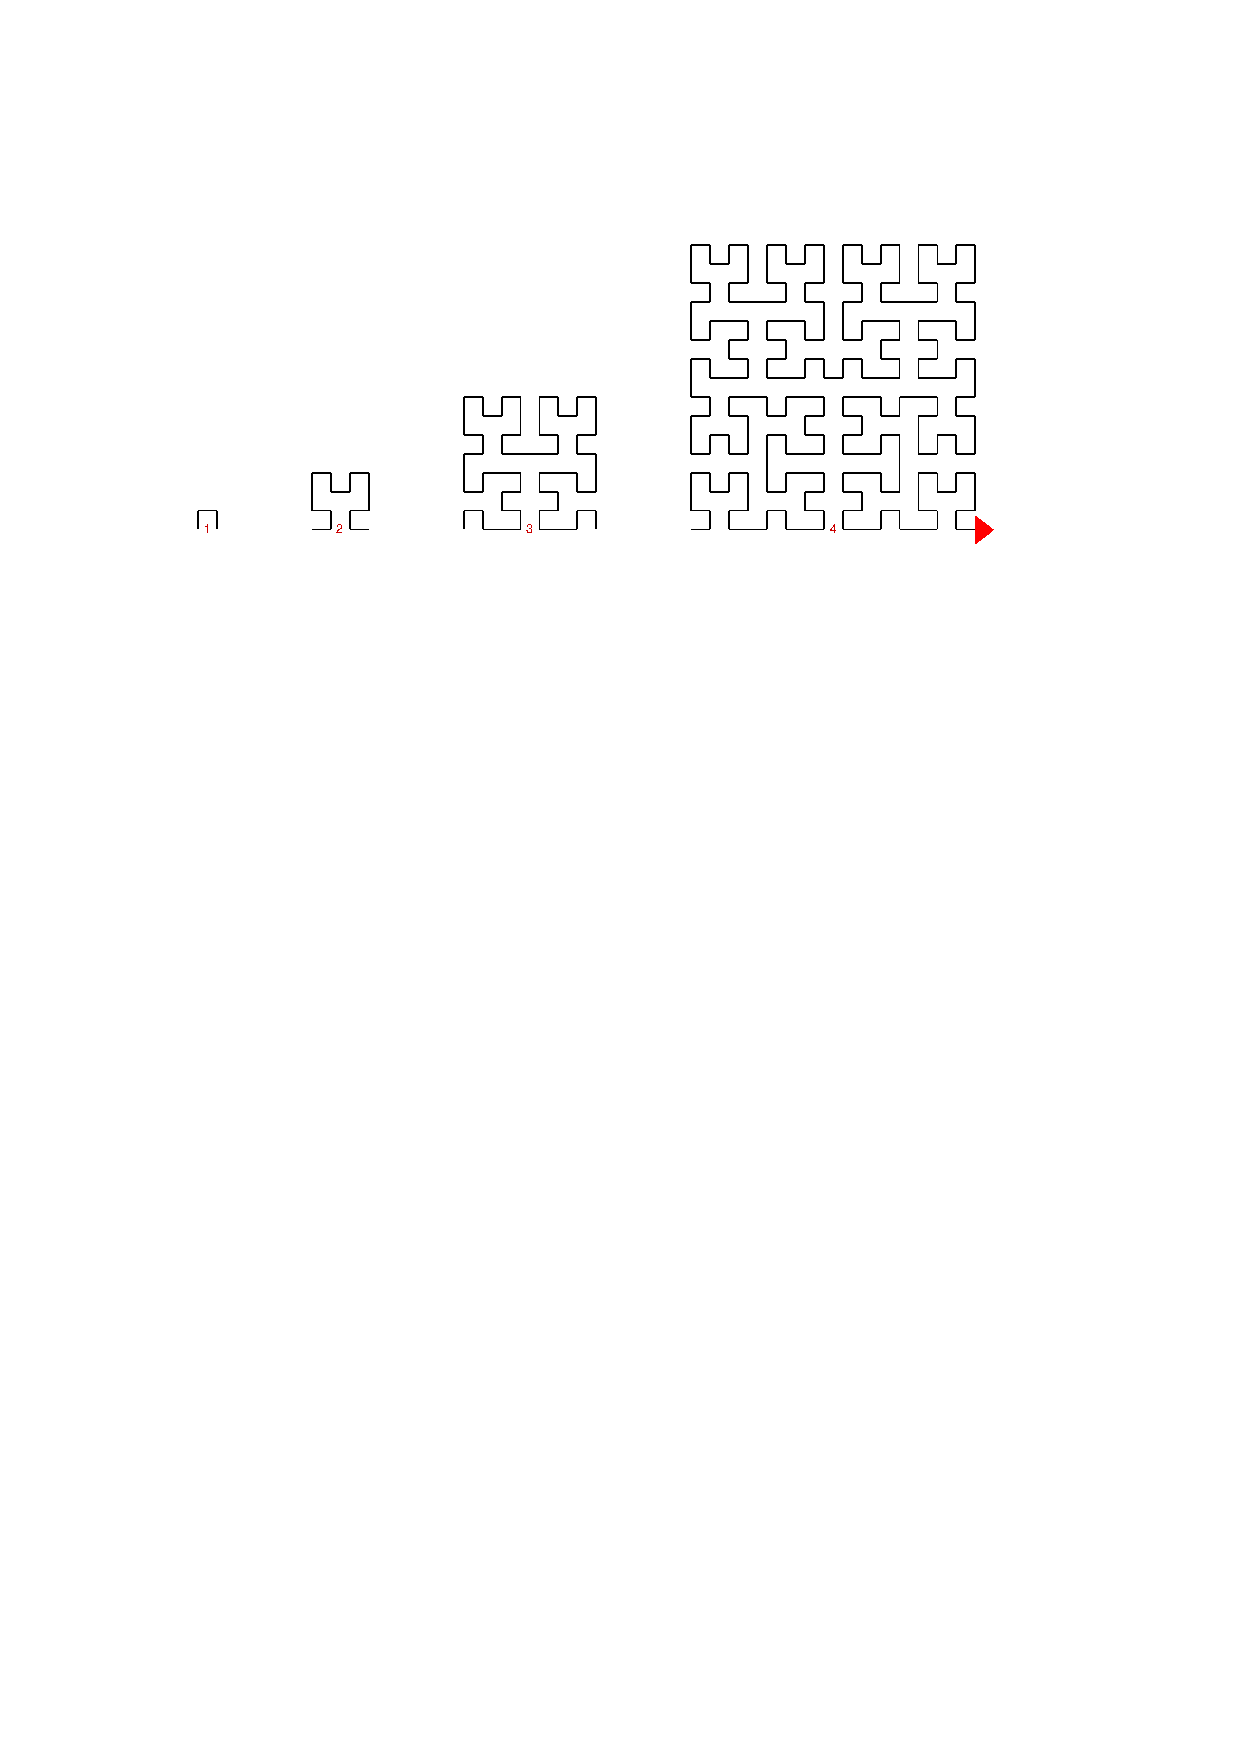
\includegraphics[width=\linewidth]{Hilbert Curve.pdf}
	\caption{Hilbert Curve (\href{https://www.cse.iitb.ac.in/~ranade/book.html}{Image Source})}
	\label{fig:hilbertcurve}
\end{figure}
\textbf{Problem Statement:}\\
Take an integer as input and draw the corresponding iteration of this fractal using \verb!turtleSim!\\
You may think along these lines
\begin{description}
	\item[Step 1]Find a simple pattern in these iterations.
	\item[Step 2]Think how can you implement this pattern in an efficient way (here think in the number of lines of code you have to write. \textbf{Word of caution}: this is just one of the possible definitions of efficient code).
	% \item[Step 3]Do you think that you need something that will implement/shorten your code?\\ How will it look like? (it’s a feature)
	\item[Step 3]Write the code!
\end{description}
In case you are stuck, here's the starter code!
\begin{tcolorbox}[breakable, enhanced, sharpish corners]%, colback = white]
	\href{https://github.com/paramrathour/CS-101/tree/main/Starter Codes/Hilbert Curve.cpp}{\textbf{Starter Code}}
\end{tcolorbox}
Feel free to discuss your thoughts.
\begin{funvideo}
\href{https://youtu.be/3s7h2MHQtxc}{Hilbert's Curve: Is infinite math useful? -- 3Blue1Brown}\\
\href{https://youtu.be/b-Fa6HtvGtQ}{Recursive PowerPoint Presentations [Gone Fractal!] -- Stand-up Maths}	
\end{funvideo}
For more interesting recursive and fractal problems, check out \hyperref[pp:lsystems]{L-Systems}.
\end{document}